\documentclass[12pt]{article}
\usepackage{amsmath}
\usepackage{mathtools}
\usepackage{bigints}
\usepackage{color}
\usepackage{parskip}
\usepackage{amssymb}
\usepackage{relsize}
\usepackage{fullpage}

\usepackage{hyperref}

	\addtolength{\topmargin}{-.5in}
	\addtolength{\textheight}{1.75in}

    \newenvironment{myindentpar}[1]%
     {\begin{list}{}%
             {\setlength{\leftmargin}{#1}}%
             \item[]%
     }
     {\end{list}}

\begin{document}
\title{Math for Business Study Guide Midterm 2}
\date{Fall 2014}
\maketitle

\textbf{NOTE:} This is intended as a study aid for the midterm. This is not an official study guide. It is just something that I create on my own in the hopes that you find it useful. The supervising professor for the course has nothing to do with the creation of this study guide. There are likely things that will be covered in the midterm that I don't put on here so it's ultimately up to you as the student to make sure you're properly prepared. However, that being said, I do try to cover the main topics and it's helpful to have one document to look at that lists most of the formulas you need to know for the midterm.

\section{Chapter 3: Exponential and Logarithm Functions}

\subsection{Exponential Functions and Their Graphs}

\textbf{Exponential Function}
\newline

\centerline{$f(x) = b^x$ \hspace{2cm} $b\neq 1$ and $b > 0$} 

\vspace{.5cm}

\centerline{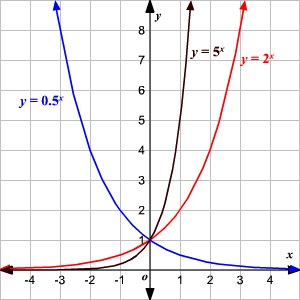
\includegraphics{ExponentialFunctionsAndGraphs.jpg}}

We say $b$ is the \textbf{base} of the exponential function.

There is a special kind of exponential function that we single out because of its significance and we call it the \textbf{Natural Exponential Function}. It is the function

\centerline{$f(x) = e^{x}$}

\newpage

\textbf{Evaluating Logarithms:}

\begin{myindentpar}{1cm}

\textbf{Evaluate the following expressions:}

\begin{enumerate}
\item $\log_{2}(8)$ 
\item $\log_{32}(2)$
\item $\log_{7}(-3)$
\item $6^{\log_{6}(8)}$

\end{enumerate}

\textbf{(1)} We ask ourselves the following question: When does $2^{y} = 8$? Well we know $2^{3} = 8$ so our answer is $\log_{2}(8) = 3$ 

\textbf{(2)} We ask ourselves the following question: When does $32^{y} = 2$? Well we know $32^{\dfrac{1}{5}} = 2$ so our answer is $\log_{32}(2) = \dfrac{1}{5}$ 

\textbf{(3)} We ask ourselves the following question: When does $7^{y} = -3$? If we think about it we should realize this can never happen so there is no solution

\textbf{(4)} There is a property in the book that says that $a^{\log_{a}(x)} = x$ so our answer is $6^{\log_{6}(8)} = 8$
\end{myindentpar}

\vspace{1cm}

\textbf{Compound Interest:}

\centerline{$A = P\Big(1 + \dfrac{r}{n}\Big)^{nt}$}

\vspace{1cm}

\textbf{Continously Compounded Interest:}

\centerline{$A = Pe^{rt}$}

\newpage

\subsection{Logarithm Functions and Their Graphs}

\textbf{Logarithm Function}
\newline

\centerline{$f(x) = \log_{b}(x)$ \hspace{2cm} $b \neq 1$ and $b > 0$} 

\vspace{.5cm}

\centerline{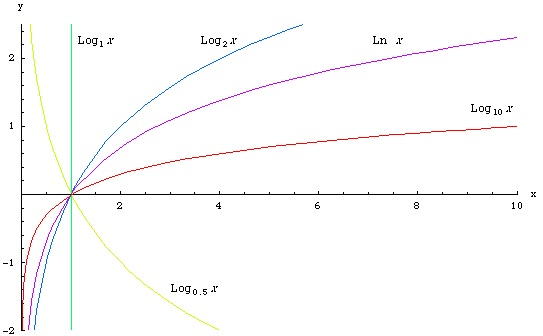
\includegraphics{LogGraph.jpg}}

Again, we call $b$ the \textbf{base} of the logarithm function. 

There is a special kind of logarithm function that we single out becaue of its significance. It is the \textbf{Natural Log Function}. It is the function
\newline

\centerline{$f(x) = \ln(x)$}

The Natural Log Function is the logarithm function with \textbf{base e} \Big($f(x) = \log_{e}(x)$\Big) and it is the \textbf{inverse} of the natural exponential function $f(x) = e^{x}$

\textbf{Note:} If you see something like $f(x) = \log(x)$ with no base, then we assume it is \textbf{log base 10}, or written out, we assume $f(x) = \log_{10}(x)$

\textbf{Logarithm to Exponential Conversion:}
\newline

\centerline{$y = \text{log}_{b}(x) \Leftrightarrow x = b^{y}$}

\textbf{Finding Domain of a Log Function:}
\newline

\centerline{Given $\text{log}_{b}(\text{STUFF})$ we set STUFF $> 0$}


\begin{myindentpar}{1cm}
\textbf{Example:} Find the domain of $\text{log}_{3}(x-3)$

\begin{myindentpar}{2cm}
- Set $x - 3 > 0 \implies x > 3$ is the domain
\end{myindentpar}
\end{myindentpar}

\newpage

\subsection{Properties of Logarithms}

\textbf{Important Properties of Exponents:}
\begin{myindentpar}{2cm}
\begin{enumerate}
\item $b^m \cdot b^n = b^{m+n}$ 
\item $(b^m)^n = b^{mn}$
\item $b^{1} = b$
\item $b^{-m} = \dfrac{1}{b^{m}}$
\item $(ab)^m = a^m \cdot b^m$
\item $\dfrac{b^{m}}{b^n} = b^{m-n}$
\item $b^{0} = 1$
\end{enumerate}
\end{myindentpar}


\textbf{Important Properties of Logs:}
\begin{myindentpar}{2cm}
\begin{enumerate}
\item $\log_{b}(1) = 0$
\item $\log_{b}(b) = 1$
\item $\log_{b}(b^{x})= x$
\item $b^{\log_{b}(x)} = x$
\item $\log_{b}(x \cdot y) = \log_{b}(x) + \log_{b}(y)$ 
\item $\log_{b}\Big(\dfrac{x}{y}\Big) = \log_{b}(x) - \log_{b}(y)$
\item $\log_{b}(x^{p}) = p \cdot \log_{b}(x)$
\end{enumerate}
\end{myindentpar}

\textbf{Change of Base:}
\newline

\centerline{$\log_{b}(M) = \dfrac{\log_{a}(M)}{\log_{a}(b)}$}

\subsection{Exponential and Logarithm Equations}

- Refer to the textbook and homework/quizzes (Sorry I had no idea how to explain this in a PDF without just typing up a bunch of examples which I didn't feel like doing)

\subsection{Exponential and Logarithm Models}

- Refer to the textbook and homework/quizzes

\newpage

\section{Chapter 8: Systems of Linear Equations and Inequalities}

\subsection{Systems of Linear Equations in Two Variables}

\begin{itemize}
\item We learned two methods for solving systems of equations in two variables:
\begin{enumerate}
\item \textbf{Substitution Method}
\item \textbf{Elimination Method}
\end{enumerate}

\item See the following examples for the difference between these two methods
\end{itemize}

\textbf{Substitution Method:}

\centerline{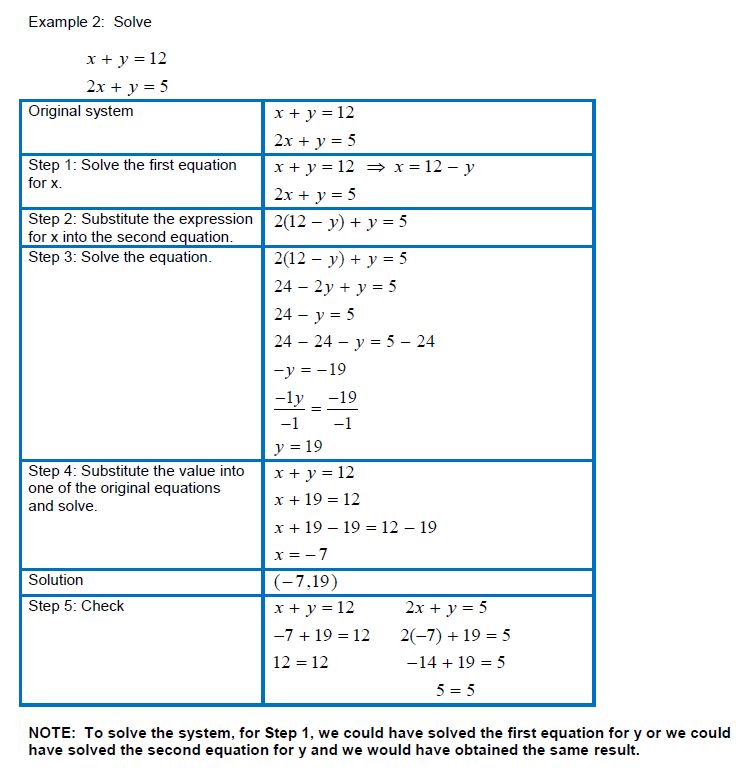
\includegraphics[scale = 0.9]{Substitution.png}}

\newpage

\textbf{Elimination Method:}

\centerline{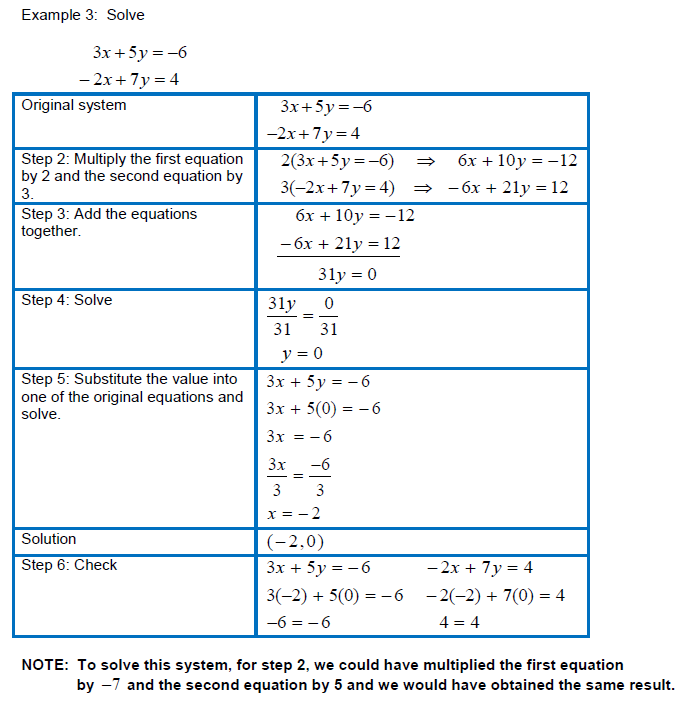
\includegraphics{Elimination.png}}

\subsection{Systems of Linear Equations in Three Variables}

- In this section we just used the elimination method for systems with three equations and three unknowns. Please refer to the textbook for this section or just go look at the Matrix Algebra section of this review. I cover the three methods we learned to solving systems of equations

\newpage

\subsection{Systems of Linear Equations and Matrices}

\textbf{Matrix:}

\begin{itemize}
\item a \textit{matrix} is a rectangular array of numbers
\item the \textit{dimension} of a matrix is the number of rows ($m$) by the number columns ($n$). A general matrix with $m$ rows and $n$ columns has dimension $m \times n$.

\textbf{Dimension:} (\# of Rows) $\times$ (\# of Columns)
\item matrices allow us to succinctly represent a large amount of information
\end{itemize}

\textbf{Augmented Matrix:}

\begin{itemize}
\item In order to solve a linear system using matrices we write a system of equations as an \textit{augmented matrix}
\item See the picture below to see how we write a system of equations as an augmented matrix:
\newline

\centerline{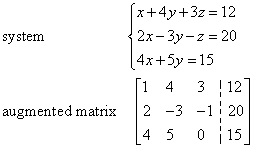
\includegraphics{AugmentedMatrix.jpg}}
\end{itemize}

Now we write the system as an augmented matrix to help solve the system for $x,y,$ and $z$. In this section we learned 2 methods for solving systems of equations:

\begin{enumerate}
\item \textbf{Gaussian Elimination with Back-Substitution}
\item \textbf{Gauss-Jordan Elimination}
\end{enumerate}

- Please refer to the next section for examples on Gaussian Elimination with Back-Substitution and Gauss-Jordan Elimination

\subsection{Matrix Algebra}

\begin{itemize}
\item \textbf{Addition:} Given two matrices $A$, $B$ of the same dimension then the sum $A + B$ is the matrix obtained by adding the corresponding entries in the two matrices
\begin{myindentpar}{1cm}
Example: 

$\begin{bmatrix}                                        
       1 & 2 & 0           \\[1em]			
       -5 & 0           & 3 \\[1em]       		
       2           & -3 & -6				
     \end{bmatrix}$
+ 			 
$\begin{bmatrix}                                        
       -3 & 7 & -2           \\[1em]			
       0 & 4           & -2 \\[1em]       		
       5           & -1 & 2				
     \end{bmatrix}$
= 
$\begin{bmatrix}                                        
       -2 & 9 & -2           \\[1em]			
       -5 & 4           & 1 \\[1em]       		
       7           & -4 & -4				
     \end{bmatrix}$
\end{myindentpar}
\item \textbf{Subtraction:} Given two matrices $A$, $B$ of the same dimension then the difference $A - B$ is the matrix obtained by subtracting the corresponding entries in the two matrices
\item \textbf{Scalar Multiplication:} Given a matrix $A$ and a number $c$ then the product $cA$ is the matrix obtained by multiplying each entry of $A$ by $c$
\end{itemize}


\begin{myindentpar}{1cm}
Example:

2 $\cdot \begin{bmatrix}                                        
       1 & 2 & 0           \\[1em]			
       -5 & 0           & 3 \\[1em]       		
       2           & -3 & -6				
     \end{bmatrix}$
= 
$\begin{bmatrix}                                        
       2 & 4 & 0           \\[1em]			
       -10 & 0           & 6 \\[1em]       		
       4           & -6 & -12				
     \end{bmatrix}$
\end{myindentpar}

\vspace{1cm}

\textbf{Matrix Multiplication:}

\begin{itemize}
\item Given two matrices, $A$, $B$, we can also find the matrix product $AB$, but we need to be careful. Matrix multiplication is NOT ALWAYS possible.
\item Given two matrices $A$, $B$ we can find the matrix product, $AB$, if the \textbf{number of columns of A is equal to the number of rows in B}
\item Given a matrix $A$ of dimension $(m \times n)$ and a matrix $B$ of dimension $(n \times k)$ AB will be a matrix of dimension $(m \times k)$
\item So if we are multiplying a $(\textcolor{red}{m} \times \textcolor{blue}{n})$ matrix $A$ by a $(\textcolor{blue}{n} \times \textcolor{red}{k})$ matrix $B$. The inner numbers (the numbers in \textcolor{blue}{blue}) will tell you whether or not matrix multiplication is possible. If it is possible, the outer numbers (numbers in \textcolor{red}{red}) tell you the dimension of the matrix AB

\begin{myindentpar}{1cm}
Example:

A = $\begin{bmatrix}                                        
       1 & 3 & -2           \\[1em]			
       -1 & 1           & 4 \\[1em]       		
       3          & 0 & -3 \\[1em]	
       2          & -4 & -6			
     \end{bmatrix}$ \hspace{1cm}
B = $\begin{bmatrix}                                        
       -1 & 2 & 0           \\[1em]			
       -5 & 2           & 3 \\[1em]       		
       0          & -1 & -3				
     \end{bmatrix}$

\vspace{1cm}

\centerline{
AB = $\begin{bmatrix}                                        
       1(-1) + 3(-5) + -2(0) & 1(2) + 3(2) + -2(-1) & 1(0) + 3(3) + -2(-3)           \\[1.5em]			
       -1(-1) + 1(-5) + 4(0) & -1(2) + 1(2) + 4(-1)           & -1(0) + 1(3) + 4(-3) \\[1.5em]       		
       3(-1) + 0(-5) + -3(0)          & 3(2) + 0(2) + -3(-1) & 3(0) + 0(3) + -3(-3)  \\[1.5em]   
       2(-1) + -4(-5) + -6(0)          & 2(2) + -4(2) + -6(-1) & 2(0) + -4(3) + -6(-3)			
     \end{bmatrix}$}

\vspace{1cm}

\centerline{
= $\begin{bmatrix}                                        
       -16 & 10& 15           \\[1.5em]			
       -4& -4 & -9 \\[1.5em]       		
       -3 & 9 & 9   \\[1.5em]   
       18 & 2 & 6			
     \end{bmatrix}$
}
\end{myindentpar}

\textbf{Note:} To find the entry in the \textbf{\textcolor{red}{first row}}, \textbf{\textcolor{blue}{first column}} of AB we multiply the corresponding entries of the \textbf{\textcolor{red}{first row of A}} by the \textbf{\textcolor{blue}{first column of B}} and add them all up.

To find the entry in the \textbf{\textcolor{red}{first row}}, \textbf{\textcolor{blue}{second column}} of AB we multiply the corresponding entries of the \textbf{\textcolor{red}{first row of A}} by the \textbf{\textcolor{blue}{second column of B}} and add them all up

We can continue on in this fashion:

i.e. To find the...

\textbf{\textcolor{red}{First row}}, \textbf{\textcolor{blue}{third column}} of AB $\rightarrow$ multiply the \textbf{\textcolor{red}{first row of A}} by the \textbf{\textcolor{blue}{third column of B}} and add

\textbf{\textcolor{red}{First row}}, \textbf{\textcolor{blue}{fourth column}} of AB $\rightarrow$ multiply the \textbf{\textcolor{red}{first row of A}} by the \textbf{\textcolor{blue}{fourth column of B}} and add

\textbf{\textcolor{red}{Second row}}, \textbf{\textcolor{blue}{first column}} of AB $\rightarrow$ multiply the \textbf{\textcolor{red}{second row of A}} by the \textbf{\textcolor{blue}{first column of B}} and add

etc...

\end{itemize}

\textbf{Identity Matrix:}
\begin{itemize}
\item the \textbf{Identity Matrix} is a special type of matrix with $1's$ along the main diagonal and zeros everywhere else
\item it is always a square matrix (the number of rows = number of columns of the identity matrix)
\item given a matrix $A$ and the identity matrix $I$, the product of $AI = A$ (provided they are of appropriate dimension). So to give an analogy, multiplying a matrix by the identity matrix is like multiplying a number times $1$
\end{itemize}

\vspace{.5cm}

\begin{myindentpar}{1cm}
\centerline{
\textbf{3x3 Identity Matrix:}}
\vspace{.5cm}
\centerline{
$\begin{bmatrix}                                        
       1 & 0& 0           \\[.5em]			
       0& 1 & 0 \\[.5em]       		
       0 & 0 & 1   		
     \end{bmatrix}$}
\end{myindentpar}

\newpage

\textbf{Solving Linear Systems}
\begin{itemize}
\item We learned how to solve two types of linear systems: 

\begin{enumerate}

\item $2$ equations and $2$ unknowns
\newline

\centerline{$a_{1,1}x + a_{1,2}y = b_{1}$}

\vspace{.3cm}

\centerline{$a_{2,1}x + a_{2,2}y = b_{2}$}

\textbf{Note:} These are merely equations of lines. (Any two points $x$ and $y$ determine a line)
\item $3$ equations and $3$ unknowns:
\newline

\centerline{$a_{1,1}x + a_{1,2}y + a_{1,3}z  = b_{1}$}

\vspace{.3cm}

\centerline{$a_{2,1}x + a_{2,2}y + a_{2,3}z  = b_{2}$}

\vspace{.3cm}

\centerline{$a_{3,1}x + a_{3,2}y + a_{3,3}z = b_{3}$}

\textbf{Note:} These are equations of planes. (Any three points $x$, $y$, and $z$ determine a plane)
\end{enumerate}

\item For a (2 by 2) or a (3 by 3) system the solution will be one of three possibilities:
\begin{enumerate}
\item There will be one and only one solution
\item There will be an infinite number of solutions
\item There will be no solution
\end{enumerate}

Visually, this is what is going on in the (2 by 2) case:

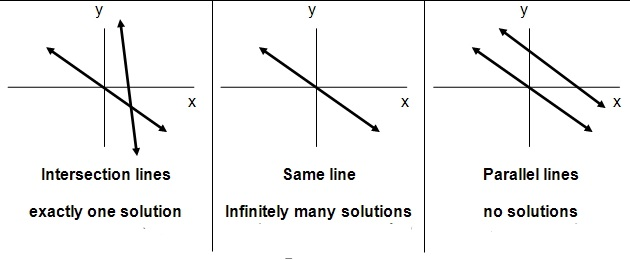
\includegraphics[scale=.7]{LinearSystemSoln.jpg}

Visually, this is what is going on in the (3 by 3) case:

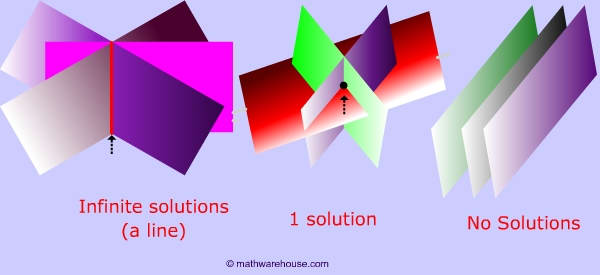
\includegraphics[scale=.5]{LinearSystemSolution3By3.jpg}

\newpage

\item to solve a linear system we learned three methods: 

\begin{enumerate}
\item \textbf{Gaussian Elimination with Back-Substitution}
\item\textbf{Gaussian-Jordan Elimination} 
\item\textbf{Inverse Matrix Method}
\end{enumerate}
All methods are very similar and they involve augmented matrices and performing row operations on the augmented matrix
\end{itemize}


\textbf{Row Operations}
\begin{enumerate}
\item Interchange any two rows
\item Multiply any row by a nonzero number
\item Add or subtract a multiple of any row to another row
\end{enumerate}

\textbf{Example of Gaussian Elimination with Back-Substitution:}

\centerline{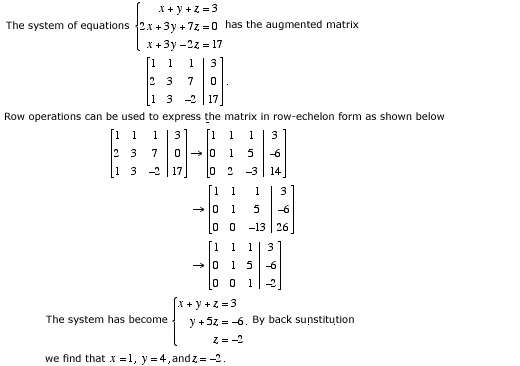
\includegraphics{GaussianElimination.jpg}}

\newpage

\textbf{Example of Gaussian-Jordan Elimination:}

\centerline{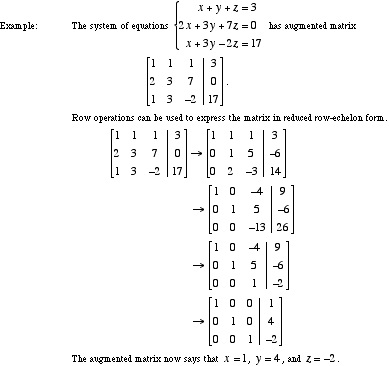
\includegraphics{GaussElim.jpg}}

\textbf{Inverse Matrix Method:}

\begin{itemize}
\item Given a linear system of $3$ equations and $3$ unknowns:
\newline

\centerline{$a_{1,1}x + a_{1,2}y + a_{1,3}z  = b_{1}$}

\vspace{.3cm}

\centerline{$a_{2,1}x + a_{2,2}y + a_{2,3}z  = b_{2}$}

\vspace{.3cm}

\centerline{$a_{3,1}x + a_{3,2}y + a_{3,3}z = b_{3}$}

\item we can write this in \textbf{matrix form} $AX = B$:
\newline

\centerline{
$\begin{bmatrix}                                        
       a_{1,1} & a_{1,2}& a_{1,3}           \\[1em]			
       a_{2,1}& a_{2,2} & a_{2,3} \\[1em]       		
       a_{3,1} & a_{3.2} & a_{3,3}   \\		
     \end{bmatrix}$
$\begin{bmatrix}                                        
       x           \\[1em]			
       y  \\[1em]       		
       z \\		
     \end{bmatrix}$
$= \begin{bmatrix}                                        
       b_{1}           \\[1em]			
       b_{2}  \\[1em]       		
       b_{3} \\		
     \end{bmatrix}$}

\item to solve this we want to find the inverse matrix of $A$ which we denote by $A^{-1}$. Once we have $A^{-1}$ we multiply $A^{-1}B$ which gives us $X$. 

\item the general idea is to start with an augmented matrix with the matrix of coefficients ($A$) on the left and the ($3 \times 3$) Identity matrix on the right:

\[
\left[
\begin{array}{ccc|ccc}
a_{1,1} & a_{1,2} & a_{1,3} & 1 & 0 & 0 \\
a_{2,1} & a_{2,2} & a_{2,3} & 0 & 1 & 0 \\
a_{3,1} & a_{3,2} & a_{3,3} & 0 & 0 & 1 \\
\end{array}
\right]
\]

and then perform a bunch of row operations to get it in the form:

\[
\left[
\begin{array}{ccc|ccc}
1 & 0 & 0 & a_{1,1}^{-1} & a_{1,2}^{-1} & a_{1,3}^{-1} \\[1em]
0 & 1 & 0 & a_{2,1}^{-1} & a_{2,2}^{-1} & a_{2,3}^{-1} \\[1em]
0 & 0 & 1 & a_{3,1}^{-1} & a_{3,2}^{-1} & a_{3,3}^{-1} \\
\end{array}
\right]
\]

where we now have the ($3 \times 3$) Identity matrix on the left and the inverse matrix ($A^{-1}$) is on the right. See the following example of how to find the inverse of a matrix $A$.
\end{itemize}

\textbf{Example of Finding Matrix Inverse:}

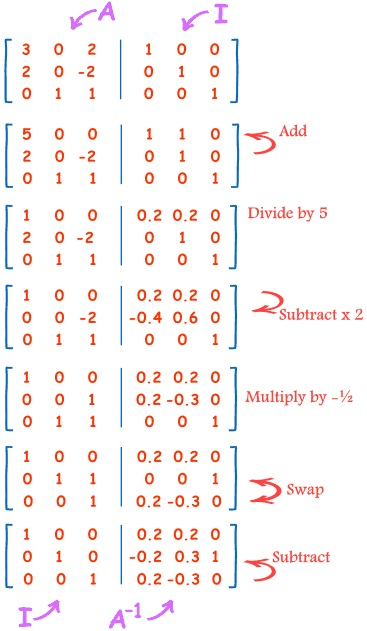
\includegraphics{InverseMatrixMethod.jpg}

\textbf{Internet Links:}
\begin{itemize}
\item \href{http://math.uww.edu/~mcfarlat/matrix.htm}{Matrix Inverse Method Example}
\item \href{https://www.youtube.com/watch?v=Re1F4d24Fxc}{PatrickJMT 2x2 Matrix Inverse Method Example}
\item \href{https://www.youtube.com/watch?v=hu6B1d3vvqU}{PatrickJMT 3x3 Matrix Inverse Method Example}
\end{itemize}


\newpage


\textbf{Formula for Inverse of a $2\text{x}2$ Matrix:}
\newline

\begin{myindentpar}{1cm}
\vspace{.5cm}
\centerline{
$ A = \begin{bmatrix}                                        
       a & b           \\[.5em]			
       c& d   		
     \end{bmatrix}$}
\end{myindentpar}

\begin{myindentpar}{1cm}
\vspace{.5cm}
\centerline{
$A^{-1} = \dfrac{1}{ad-bc}\begin{bmatrix}                                        
       d & -b           \\[.5em]			
       -c& a   		
     \end{bmatrix}$}
\end{myindentpar}



\subsection{The Determinant of a Square Matrix and Cramer's Rule}

\textbf{Determinant of a $2\text{x}2$ Matrix:}
\newline

\begin{myindentpar}{1cm}
\vspace{.5cm}
\centerline{
$ A = \begin{bmatrix}                                        
       a & b           \\[.5em]			
       c& d   		
     \end{bmatrix}$}
\end{myindentpar}

\vspace{.5cm}
\centerline{$\text{Det}(A) = |A| = ad - bc$}

\textbf{Determinant of a $3\text{x}3$ Matrix:} (Expanded along Row 1)
\newline

\centerline{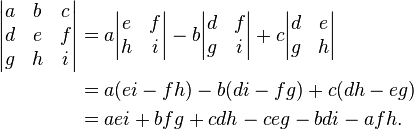
\includegraphics[scale = 0.8]{DeterminantRow1.png}}

\textbf{Determinant of a $4\text{x}4$ Matrix:} (Expanded along Row 1)
\newline

\centerline{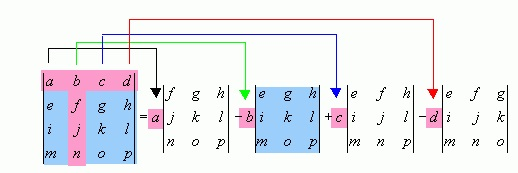
\includegraphics{Determinant4by4.jpg}}

\newpage

\textbf{Example of Finding the Determinant of a 2x2 Matrix:}

\centerline{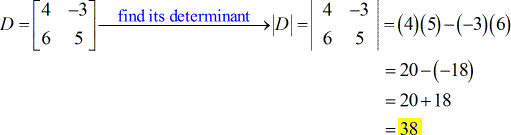
\includegraphics[scale = 0.7]{Determinant2By2Example.png}}

\textbf{Example of Finding the Determinant of a 3x3 Matrix:}

\centerline{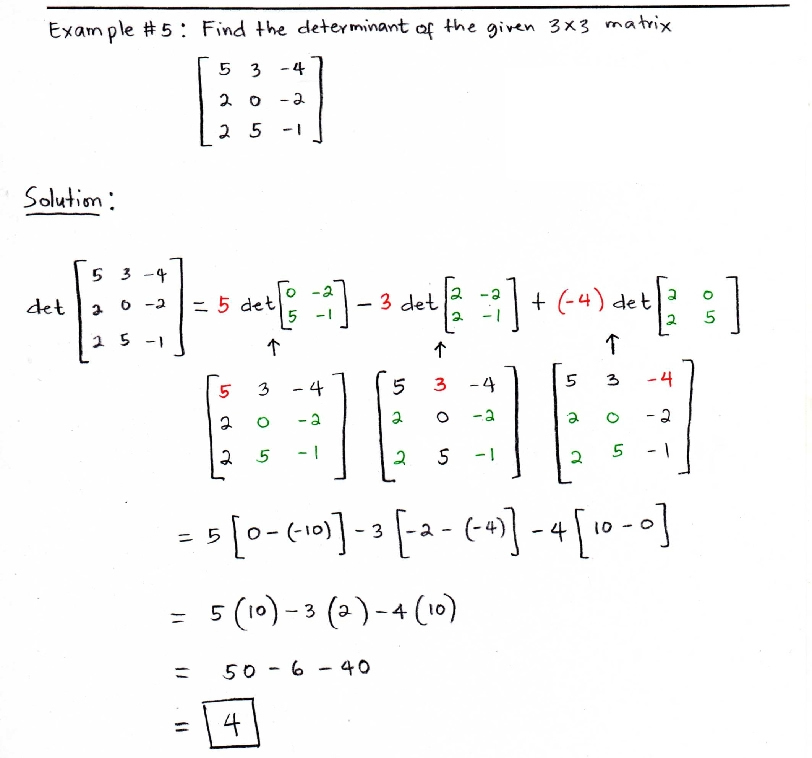
\includegraphics[scale = 0.6]{Determinant3By3Example.jpg}}

\newpage

\textbf{Example 2 of Finding the Determinant of a 3x3 Matrix:}

\centerline{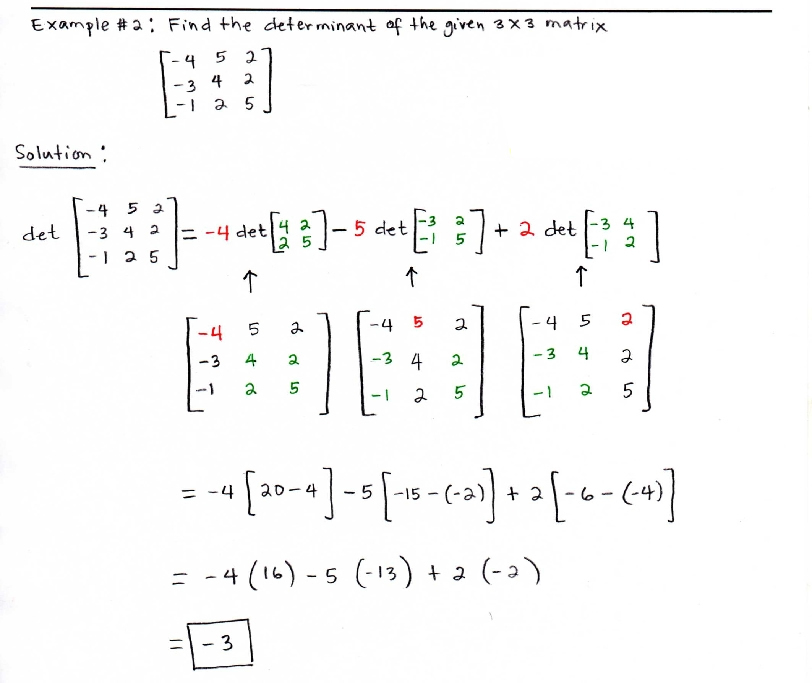
\includegraphics[scale = 0.6]{Determinant3By3Example2.jpg}}


\textbf{Cramer's Rule:}

\begin{itemize}
\item Another method for solving systems of equations
\item We learned Cramer's Rule for 2x2 matrices and for 3x3 matrices
\end{itemize}

\newpage

\textbf{Cramer's Rule for 2x2 Matrices:}
\newline

\centerline{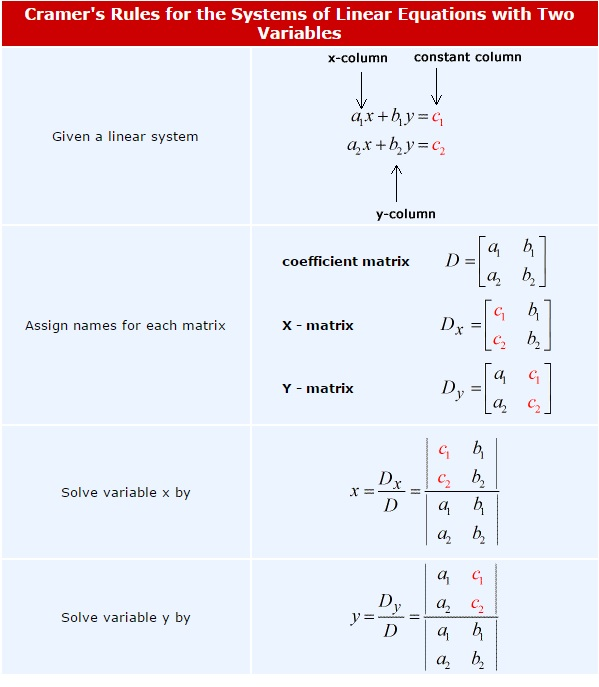
\includegraphics{CramersRule2By2.jpg}}

\newpage

\textbf{Cramer's Rule for 3x3 Matrices:}
\newline

\centerline{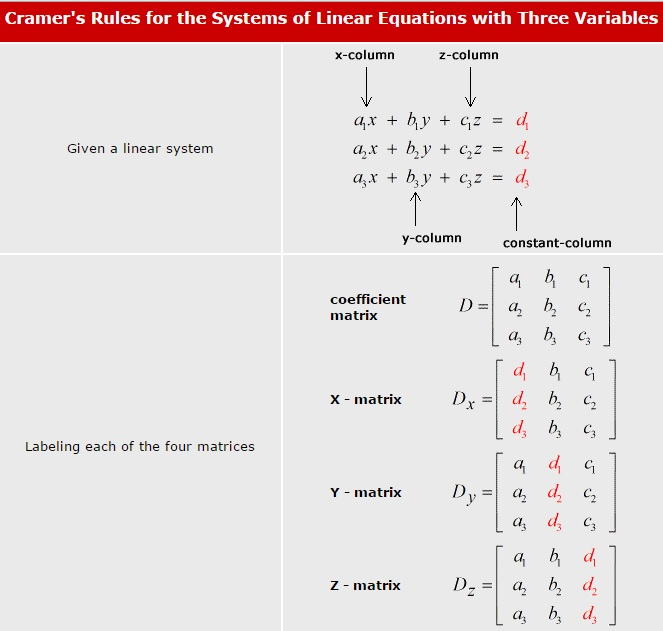
\includegraphics{CramersRule3By31.jpg}}

\textbf{CONTINUED ON NEXT PAGE!!!}

\centerline{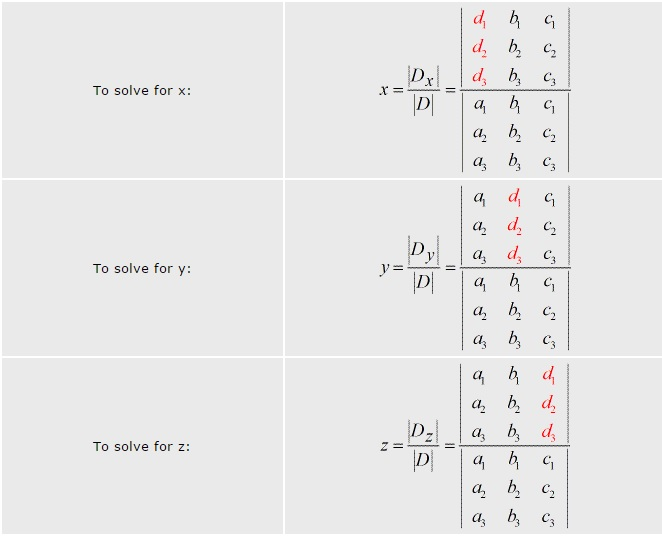
\includegraphics{CramersRule3By32.jpg}}

\textbf{Internet Links:}
\begin{itemize}
\item \href{https://www.youtube.com/watch?v=cidMyv6L7Gs}{Guru Cramer's Rule 2x2 Example}
\item \href{http://www.chilimath.com/algebra/advanced/cramers/2x2.html}{Cramer's Rule for 2x2 and 3x3 Matrices Examples and Solutions}
\item \href{https://www.youtube.com/watch?v=TtxVGMWXMSE}{PatrickJMT Cramer's Rule 3x3 Example 1}
\item \href{https://www.youtube.com/watch?v=iMQRo0tHORw}{PatrickJMT Cramer's Rule 3x3 Example 2}

\end{itemize}














\end{document}